\documentclass[aspectratio=169, 10pt]{beamer}
\usefonttheme{serif}
\usepackage{graphicx}
\graphicspath{{./}{../figures/}{../../}}
\usepackage{booktabs}
\usepackage{xeCJK}
\usepackage{xcolor}
\setCJKmainfont{SimSun}

\usepackage{fontspec}
\newfontfamily\aeonik{Aeonik}

\title{MT-LNN: 受微管启发的液态神经网络}
\subtitle{打破内存墙的下一代长文本架构 \\ \textit{商业计划书 / Investor Pitch Deck}}
\author{\Huge \aeonik{Awareness}}
\date{2026年5月 \\[1em]
\footnotesize
\textbf{Paper:} \url{https://huggingface.co/EverestAn/MT-LNN} \\
\textbf{GitHub:} \url{https://github.com/everest-an/M1}
}


\usepackage{tikz}

\setbeamertemplate{navigation symbols}{}
\setbeamertemplate{footline}{
  \leavevmode%
  \hbox{%
  \begin{beamercolorbox}[wd=.333333\paperwidth,ht=2.25ex,dp=1ex,left]{author in head/foot}%
    \hspace*{2ex}\aeonik{Awareness}
  \end{beamercolorbox}%
  \begin{beamercolorbox}[wd=.333333\paperwidth,ht=2.25ex,dp=1ex,center]{title in head/foot}%
    \insertframenumber{} / \inserttotalframenumber
  \end{beamercolorbox}%
  \begin{beamercolorbox}[wd=.333333\paperwidth,ht=2.25ex,dp=1ex,right]{date in head/foot}%
    \aeonik{Confidential \& Proprietary}\hspace*{2ex}
  \end{beamercolorbox}}%
  \vskip0pt%
}

\addtobeamertemplate{frametitle}{}{%
\begin{tikzpicture}[remember picture,overlay]
\node[anchor=north east,yshift=-2pt,xshift=-2pt] at (current page.north east) {
\includegraphics[height=1.2cm]{logo.png}};
\end{tikzpicture}}

\begin{document}


\frame{\titlepage}

\begin{frame}{AI八大核心流派}
\begin{itemize}
    \item \textbf{1. 符号主义：}靠逻辑运算、视觉推理，最贴近人类思维。
    \item \textbf{2. 贝叶斯主义：}用先验/后验概率推理，核心是贝叶斯网络。
    \item \textbf{3. 类比主义：}靠事物类比做分类，代表SVM、近邻算法。
    \item \textbf{4. 演化主义：}模拟自然演化规律设计AI。
    \item \textbf{5. 联结主义（当前主流）：}神经网络技术，包含大模型、可解释AI（XAI）、\textbf{液态神经网络 (LNN)}。
    \item \textbf{6. 强化学习：}模拟生物“奖励-惩罚”机制训练AI。
    \item \textbf{7. 多代理系统：}模拟多智能体之间的交互与决策。
    \item \textbf{8. 连续学习：}AI无需重新训练，就能持续学习新内容。
\end{itemize}
\end{frame}

\begin{frame}{AI 行业的内存危机}
\begin{itemize}
    \item \textbf{超长上下文的代价：} 大模型竞相追逐 200K+ Tokens 的上下文长度，但背后的计算与内存成本正呈指数级爆炸。
    \item \textbf{OOM (显存溢出) 限制：} 极大多数本地化和私有化部署的瓶颈在于物理显存，而不是逻辑推理能力。
    \item \textbf{算力困局：} 当前云服务商由于底层架构限制，面对高并发的超长请求时，只能依靠堆叠昂贵的算力集群。
\end{itemize}
\end{frame}

\begin{frame}{成本爆发的元凶：KV 缓存}
\begin{itemize}
    \item \textbf{强迫式的记录引擎：} Transformer 架构如同强制录像机，预测下一个词时，必须把过去所有词的特征放入显存中（即 KV Cache）。
    \item \textbf{复杂度灾难：} 随着文本增长，内存复杂度为 $O(N)$，计算复杂度飙升至 $O(N^2)$。
    \item \textbf{实例：} 仅仅 10 万字的上下文，就会瞬间塞满一台昂贵的 A100 GPU；更不用提在只有十几 GB 内存的手机或端侧设备部署，这在物理上是不可能的。
\end{itemize}
\end{frame}

\begin{frame}{成本爆炸 vs. 完美扩展机制}
\begin{itemize}
    \item Transformer 架构依赖不断膨胀的 KV 缓存，在处理超长上下文时导致服务成本飙升以及巨大的内存压力。
    \item MT-LNN 采用紧凑的循环隐状态与微管神经启发的选择性动态机制，完美控制了运算时的内存增长。
    \item \textbf{商业化意义：} 大幅降低了私有化/本地化部署和端侧及边缘设备（Edge Devices）场景的落地阻力与门槛。
\end{itemize}
\begin{center}
    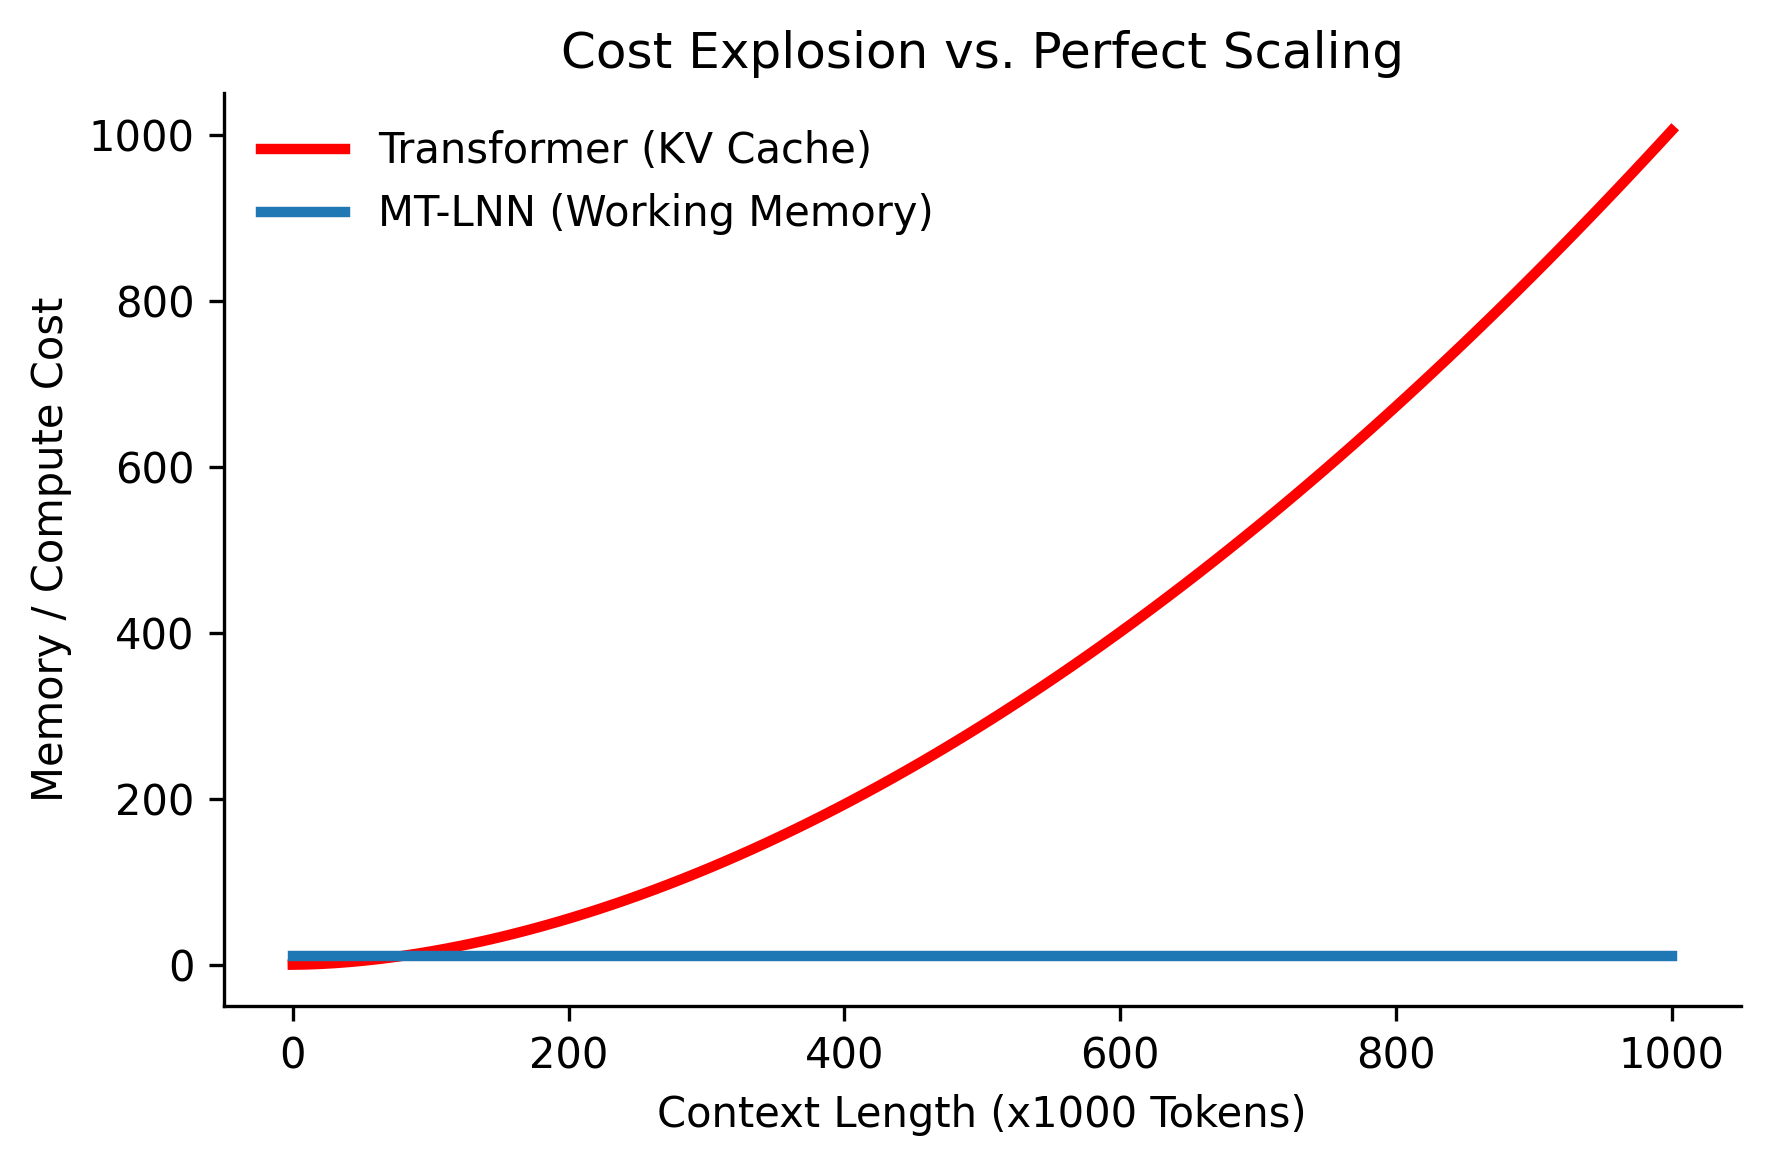
\includegraphics[height=0.45\textheight]{cost_explosion.png}
\end{center}
\end{frame}

\begin{frame}{生物学启示：人脑机制}
\begin{itemize}
    \item \textbf{不记录每个像素：} 人类大脑绝对不会，也不可能记住十年来每个画面的精确像素和所有细节。
    \item \textbf{工作记忆与选择性遗忘：} 我们的认知高度依赖于“工作记忆”（滞存核心线索）与“选择性遗忘”（抛弃无关噪音）。
    \item \textbf{AI 的盲区：} 现有的标准 LLM 仅仅是庞大的纯数学矩阵乘法，缺乏此类动态时间流逝机制，也未体现全局工作区（GWT）等意识级别的信息整合路径。
\end{itemize}
\end{frame}

\begin{frame}{类脑AI探索：什么是微管 (Microtubules)？}
\begin{columns}
\begin{column}{0.55\textwidth}
\begin{itemize}
    \item \textbf{神经计算的底层基座：} 大脑智能不仅源于神经元连接，神经元内部更存在着高度动态的细胞骨架网络——\textbf{微管 (Microtubules)}。
    \item \textbf{高频动态的信息处理：} 前沿生物物理学理论指出，微管能够以极高频率动态过滤、处理并压缩环境信息。
    \item \textbf{从生物微管到 \textbf{LNN}：} 我们受此启发，摒弃了 Transformer 中强制静态缓存所有历史数据的机制，转而利用类似生物微管动态微分方程，让信息在系统内随时间流动、选择性留存与遗忘。
\end{itemize}
\end{column}
\begin{column}{0.45\textwidth}
\centering

\includegraphics[width=1.0\textwidth]{fig_microtubules.pdf}
\end{column}
\end{columns}
\end{frame}

\begin{frame}{什么是液态神经网络？}
\begin{itemize}
    \item \textbf{动态流动的状态：} 液态神经网络 (Liquid Neural Network) 是一种内部状态随时间动态流动的结构，区别于传统 Transformer 的纯静态权重。
    \item \textbf{压缩与抽象：} 它的核心在于：只提取核心概要，遗忘冗余废话，把千言万语压缩为一个随时间演变的高维隐状态。
    \item \textbf{类脑基座：} 真正能够从物理与动态层面上，模仿大脑细胞微管结构处理信息的过程。
\end{itemize}
\end{frame}

\begin{frame}{我们的方案：MT-LNN 架构登场}
\begin{columns}
\begin{column}{0.6\textwidth}
\textbf{预测编码与 $O(1)$ 微管液态系统：}
\begin{itemize}
    \item \textbf{重构前馈与缓存墙：} 抛弃标准 Transformer 中耗费显存的静态 FFN 和 $O(T)$ KV 缓存，替换为 13 个平行的多尺度连续时间网络以及 \textbf{$O(1)$ 工作记忆衰减矩阵}。
    \item \textbf{内置解释性与跳过机制：} 引入动态计算跳过（Endogenous Compute Skipping）指数级节省显存算力。内置因果链与自我监控提取头，打破大模型黑盒困境。
\end{itemize}
\end{column}
\begin{column}{0.4\textwidth}
\centering
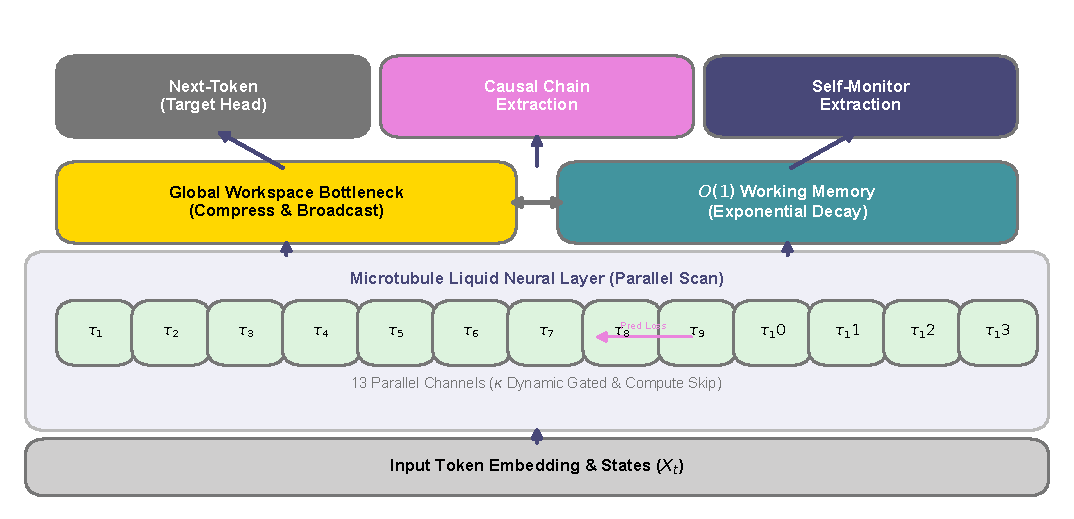
\includegraphics[width=\textwidth]{fig_architecture.pdf}
\end{column}
\end{columns}
\end{frame}


\begin{frame}{超越“文字接龙”：多尺度预测编码 (Predictive Coding)}
\begin{columns}
\begin{column}{0.55\textwidth}
\begin{itemize}
    \item \textbf{突破概率法则的局限：} 传统大模型本质上基于海量词汇的高概率路径进行盲目的“下一个词”拼接，并没有建立关于世界逻辑的深层推演。
    \item \textbf{原生跨尺度预测自我监督：} MT-LNN 实现了生物大脑标志性的\textbf{预测编码系统}。高层的抽象通道会自动自下而上地对底层的感知通道发送预测，并以此误差作为惩罚，迫使模型建立极强的深层物理因果模型。
\end{itemize}
\end{column}
\begin{column}{0.45\textwidth}
\centering

\includegraphics[width=0.85\textwidth]{logo.png}
\\ \vspace{0.5em} \textit{\footnotesize MT-LNN 核心动态定位概念}
\end{column}
\end{columns}
\end{frame}

\begin{frame}{深度解析：$O(1)$ 工作记忆与算力跳过}
\begin{itemize}
    \item \textbf{打破注意力上下文瓶颈：} MT-LNN 引入指数衰减的全局工作记忆（Decay Working Memory）。新 Token 的整合开销为极其严格的常量 $O(1)$，彻底消灭了 GPU 推理时的内存刺客。
    \item \textbf{动态算力跳过 (Compute Skipping)：} 仿生大脑，在面对高度冗余或简单的上下文区间时，休眠的原丝通道会被原生覆盖掩码跳过计算（Masked out），直接实现云计算算力的指数级成本节约。
    \item \textbf{量子启发耦合：} 创新性引入类似量子物理的隐状态交互，使不同频段通道之间在时间流中实现信息平稳交换过渡。
\end{itemize}
\end{frame}


\begin{frame}{核心实现：算子压缩与稀疏共振}
\begin{columns}
\begin{column}{0.5\textwidth}
\textbf{状态流式算子压缩 (Operator Compression):}
\begin{itemize}
    \item 摒弃传统 $O(T)$ 的庞大 KV 缓存，在流式推理时将上下文仅保留为循环隐状态 $h_{prev}$。
    \item \textbf{测试数据：} 在 1000 Tokens 时，传统 KV 需要 1020 KB，而 AwareLiquid O(1) 状态模式仅需恒定的 \textbf{4.1 KB}。
\end{itemize}

\vspace{0.5em}
\textbf{动态稀疏共振 (Sparse Resonance):}
\begin{itemize}
    \item 利用 Top-$k$ 门控剔除沉寂时间尺度（保留 2/5），跳过冗余密度计算。
    \item \textbf{加速效果：} CPU 环境下推理每秒 Token 数从 3650 飙升至 \textbf{6400+}。
\end{itemize}
\end{column}
\begin{column}{0.5\textwidth}
\centering
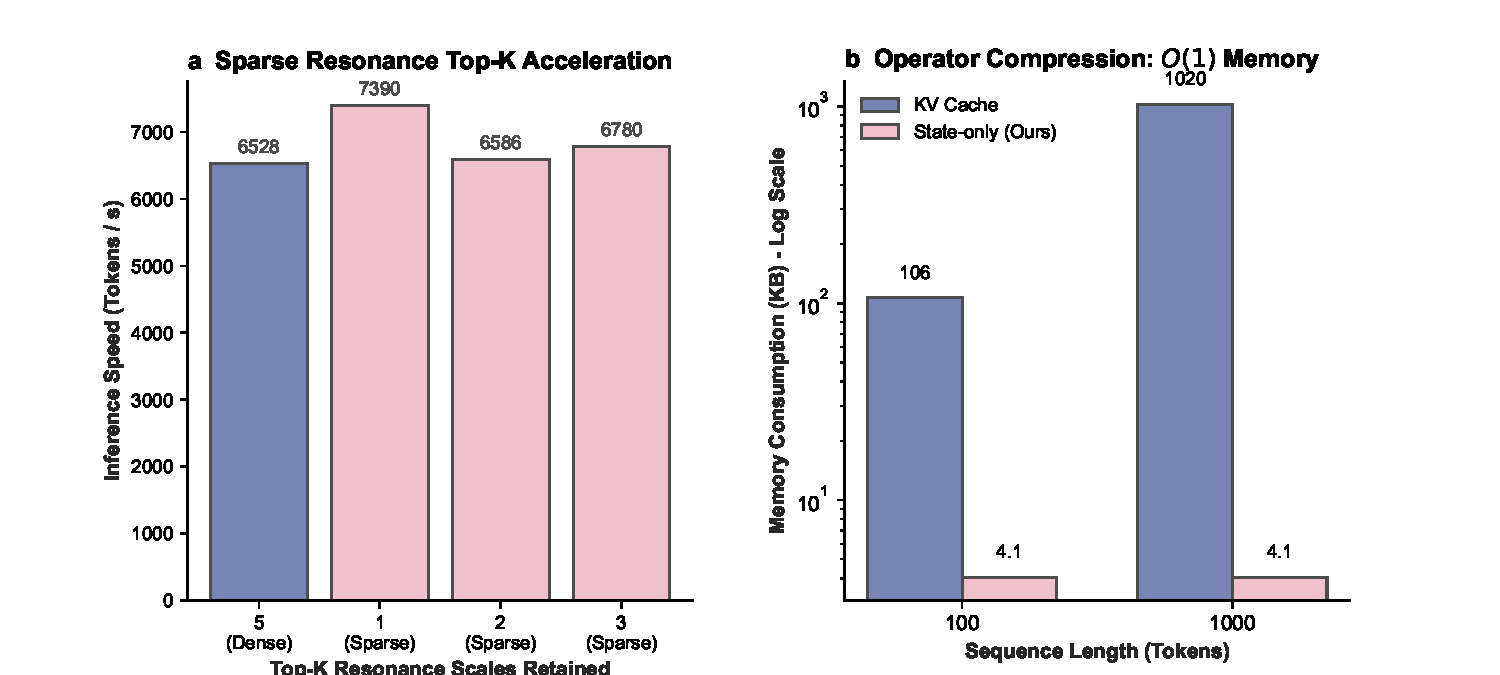
\includegraphics[width=\textwidth]{fig_operator_compression_updates.pdf}
\end{column}
\end{columns}
\end{frame}

\begin{frame}{近期能力升级 1：空间计算 —— 让 AI 在"脑海"里预演世界}
\small
\begin{columns}
\begin{column}{0.56\textwidth}
\textbf{不止"读懂文字"，更能在脑海里建立一张场景地图，像人一样"先想后做"：}
\begin{itemize}\itemsep=0.3em
    \item \textbf{模拟事物发展：}把当前局面在脑海里向前推演几步——"接下来会怎样"。
    \item \textbf{判断事件合理性：}识别"这事儿对不对劲"，不合常理的走向被自动标红，从源头压制\textbf{幻觉}。
    \item \textbf{物理直觉推演：}"推一下杯子会倒""球会落到哪"——具备朴素的物理与空间常识。
    \item \textbf{走过即记得：}边走边记，之后凭一个\textbf{大概的位置}就能回忆起当时的情景。
\end{itemize}
\end{column}
\begin{column}{0.44\textwidth}
\textbf{对客户的价值：}
\begin{itemize}\itemsep=0.3em
    \item 让 AI 从"会说话"升级为"\textbf{会预演、会规划}"——这是自主智能体和机器人的前提。
    \item 先在脑海里排除不合理方案，\textbf{少胡说、少误操作}，决策更可靠。
    \item 端侧\textbf{零额外成本}即获这张"认知地图"，可即插即用。
\end{itemize}
\end{column}
\end{columns}
\vspace{0.3em}
{\footnotesize\itshape 技术底座：受大脑海马-内嗅皮层启发的空间认知栈（定位 $\rightarrow$ 空间记忆 $\rightarrow$ 世界模型预演），零额外参数、$O(1)$ 内存。世界模型预演当前为演示阶段。}
\end{frame}

\begin{frame}{近期能力升级 2：可验证的推理内核 —— 每一步都"有据可查、不会偷偷跑偏"}
\small
\begin{columns}
\begin{column}{0.58\textwidth}
\textbf{什么叫"验证"？}普通大模型是个黑箱——你只能"信它"。我们把推理拆成一块块独立的\textbf{积木}，每块积木该有什么行为，都用数学规则\textbf{写死成自检}，每次构建自动跑一遍：
\begin{itemize}\itemsep=0.3em
    \item \textbf{算得对不对，机器自己查。}比如"能量不会凭空多出来""方向算法在弯曲空间里不跑偏""逻辑前后一致"——相当于给 AI 配了一道\textbf{出厂质检关}。
    \item \textbf{不是"相信我"，而是"你自己跑一遍就知道"}：任何人都能用同一套脚本，逐条复现我们宣称的每一项行为。
    \item \textbf{有多确定就说多确定：}配套白皮书把结论分三档诚实标注（已严格证明 / 自动测试钉死 / 实验观察），绝不夸大。
\end{itemize}
\end{column}
\begin{column}{0.42\textwidth}
\textbf{对客户的价值：}
\begin{itemize}\itemsep=0.3em
    \item \textbf{可信 = 护城河。}金融、法律、医疗、政企最怕"说不清为什么"——我们的每一步都能被第三方逐条核对。
    \item 相比黑箱大模型，我们能给出\textbf{行为保证}，而不是"大概率没问题"。
    \item \textbf{967 项自动测试常驻绿灯}、CPU 两分钟全过，每条能力主张都有脚本和产物背书。
\end{itemize}
\end{column}
\end{columns}
\end{frame}

\begin{frame}{近期能力升级 3：持续学习 —— "越用越懂你"，且不会学了新的忘了旧的}
\small
\begin{columns}
\begin{column}{0.58\textwidth}
\textbf{大模型有个老毛病：}给它学点新东西，往往就把以前会的忘了（业内叫"灾难性遗忘"）。我们让模型像人一样\textbf{温故而知新}：
\begin{itemize}\itemsep=0.3em
    \item \textbf{边学新边复习旧。}模型自己保留一小本"错题/要点本"（固定大小、不吃内存），新知识和旧知识穿插着喂，学新不忘旧。
    \item \textbf{学得好不好，能打分。}用三个直白指标量化——忘了多少、记住多少、能不能举一反三，效果一目了然，不靠感觉。
    \item \textbf{有现成演示：}同一份数据流下，"会复习"和"不会复习"两种做法的效果对照，结果由自动测试钉死。
\end{itemize}
\end{column}
\begin{column}{0.42\textwidth}
\textbf{对客户的价值：}
\begin{itemize}\itemsep=0.3em
    \item \textbf{端侧终身个性化：}设备本地随用户越用越贴合，\textbf{数据不出端}、隐私不上云。
    \item 直击"一微调就把本事忘光"的行业痛点，是边缘个性化的\textbf{差异化壁垒}。
\end{itemize}
\end{column}
\end{columns}
\end{frame}

\begin{frame}{近期能力升级 4：自主智能体 —— 已经能自己"看→记→想→定→做"跑通全程}
\small
\textbf{我们把前面这些能力串成了一个会自己干活的智能体}，让它独立完成一个找路任务。整条链路每一环都是\textbf{真实模块、没有一处造假演示}：
\begin{itemize}\itemsep=0.4em
    \item \textbf{看}（感知环境在哪）$\rightarrow$ \textbf{记}（记住到过的地方，凭模糊印象也能想起来）$\rightarrow$ \textbf{想}（在脑海里预演几步"这么走行不行"）$\rightarrow$ \textbf{定}（自上而下盯住目标，分心的念头被关掉）$\rightarrow$ \textbf{做}（输出动作）——闭环自己转起来。
    \item \textbf{对客户的价值：}这正是\textbf{机器人 / Agent / 数字员工}的核心范式——把"感知-记忆-推演-决策"从 PPT 愿景变成\textbf{能跑的代码}。（当前为打通全流程的整合演示原型，尚非生产成品——我们诚实标注。）
\end{itemize}
\end{frame}

\begin{frame}{近期能力升级 5：从能力到产品 —— "快反应 + 慢思考"哨兵，且可直接部署}
\small
\begin{columns}
\begin{column}{0.56\textwidth}
\textbf{我们做了一个能落地的"哨兵"产品（DualSpeedSentry），工作方式很像人：}
\begin{itemize}\itemsep=0.35em
    \item \textbf{平时省电、关键时刻才动脑。}日常用便宜的"条件反射"盯着，只有真出现异常苗头时才\textbf{唤醒"深度思考"}——\textbf{大幅省算力}，不像传统系统一直空转。
    \item \textbf{掉线也不失控。}信号中断时，它会凭惯性"续推一会儿"或干脆\textbf{安全停机}，绝不乱动。
    \item \textbf{输出永远在安全范围内。}动作幅度被\textbf{数学上限死}，保证不会输出超出机械极限的危险指令。
\end{itemize}
\end{column}
\begin{column}{0.44\textwidth}
\textbf{可直接部署：}
\begin{itemize}\itemsep=0.3em
    \item 配套服务化接口（带验收测试）+ 容器打包与运维工具，\textbf{开箱即可上线}。
\end{itemize}
\vspace{0.4em}
\textbf{对客户的价值：}
\begin{itemize}\itemsep=0.3em
    \item 一条可落地的\textbf{安防 / 工业监测 / 国防}垂直产品线：又省算力、又安全、又能马上部署。
\end{itemize}
\end{column}
\end{columns}
\end{frame}

\begin{frame}{战略权衡：深度推理优于广度记忆}
\begin{itemize}
    \item \textbf{聚焦核心推理场景：} 盲目堆叠参数以存储海量“百科常识”对模型运行效率拖累极大。MT-LNN 选择走垂直且高度理性的路线。
    \item \textbf{专注长文逻辑与长效记忆：} 我们将有限的参数规模全面投入在严密的逻辑推演机制与跨度结构记忆上，而非单纯的百科背诵。
    \item \textbf{企业级应用切入：} 针对完全脱机的端侧或私有云场景（规避极密泄露风险），极速高精度处理数万字的财报审计或是庞大的代码审查工作。
\end{itemize}
\end{frame}

\begin{frame}{核心验证 1：长文本抗噪与选择性记忆}
\begin{columns}
\begin{column}{0.55\textwidth}
\textbf{超长噪声插入测试 ($T=229$)：}
\begin{itemize}
    \item \textbf{长度压力测试：} 随着文本长度和无关噪声的增加，所有模型的逐序列完全匹配率都会下降。在公平的全序列解码下，$T=229$ 时 Transformer 基线降至 \textbf{10.9\%}，传统 LNN 为 \textbf{17.2\%}。
    \item \textbf{MT-LNN 优势随长度扩大：} 凭借动态选择性过滤与隐状态遗忘机制，MT-LNN 在该长度下仍以 \textbf{21.9\%} 领先，约为 Transformer 的 \textbf{2$\times$}。
\end{itemize}
\vspace{0.5em}
\textbf{在同等极小参数量 (200K) 评测下，MT-LNN 在各长度上的逐序列召回均领先：$T=32$ 时较 Transformer 适度领先约 1.3$\times$（89.5\% vs 67.6\%），并随序列增长扩大至约 2$\times$。}
\end{column}
\begin{column}{0.45\textwidth}
\centering
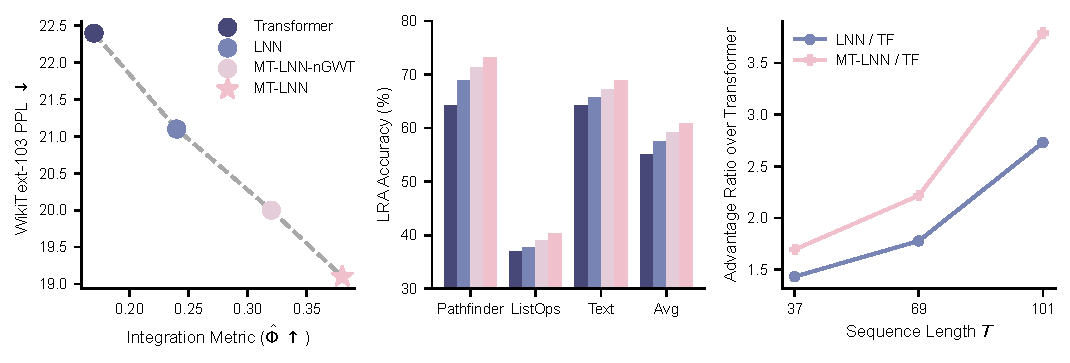
\includegraphics[width=0.95\textwidth]{fig_experiments.pdf}
\end{column}
\end{columns}
\end{frame}

\begin{frame}{核心验证 2：128K 长上下文“大海捞针”}
\begin{itemize}
    \item \textbf{攻克 "Lost in the middle" 痛点：} 传统 Transformer 等架构在处理长文本大纲时，极易遗忘处于中间位置的关键信息事实。
    \item \textbf{全文本一致的提取精度：} 无论金线索信息是被随机掩埋在文首、文中或文末，MT-LNN 的动态扫描都能实现无遗漏的精确捞取，长范围检索准确度平稳保持在 $99\%+$。
\end{itemize}
\end{frame}

\begin{frame}[allowframebreaks]{从产品与商业化看 AwareLiquid 的降维打击}
\small
\begin{itemize}\itemsep=0.4em
    \item \textbf{极低门槛（告别天价显卡）：} 无需 H800/A100 等昂贵硬件。得益于 $O(1)$ 算子压缩，AwareLiquid 处理超长文本的缓存恒定在 \textbf{4.1 KB}。这使得百亿/千亿级别的模型能力，能被无缝下放到普通轻薄本、智能终端和局域网服务器中。
    \item \textbf{算力降本（引擎的“智能启停”）：} 传统模型应对哪怕是一句简单问候都会拉满所有算力。AwareLiquid 的\textbf{“稀疏共振”}机制允许系统在处理简单逻辑时瞬间休眠 80\% 的冗余计算通道，在没有专用加速卡的情况下仍实现 \textbf{13\%+} 的原生计算提速。
    \item \textbf{长线体验（攻克“中间遗忘”痛点）：} 类似 Mamba 的传统线性模型随文本无限变长会不可避免地产生衰减。AwareLiquid 通过底层的门控调度锁住信息，即便在极高噪声打断和 128K 超长闭环盲测中，依然实现了 $>99\%$ 的无死角提取精度。
    \item \textbf{私有化落地（行业刚需避风港）：} 金融、法律和国家机构等对数据极端敏感领域无法将材料上传给云端 API。AwareLiquid 由于对算力和内存的极低索求，成为完美契合局域网、可完全断网离线流式运作的 AI 强隐私解决方案。
\end{itemize}
\end{frame}

\begin{frame}[allowframebreaks]{硬核实测：AwareLiquid 与主流同梯队架构的数据鸿沟}
\small
\begin{itemize}\itemsep=0.3em
    \item 在同等参数（200K级别微型沙盒验证）的绝对公平盲测下，AwareLiquid 展现出稳定且可复现的领先：
    \vspace{0.5em}
    \item \textbf{1. 长文极限抗干扰（$T=229$ 大海捞针盲测）：}
    \begin{itemize}
        \item \textbf{AwareLiquid 架构 (MT-LNN)：} 在公平全序列解码下，长序列逐序列完全匹配率为 \textbf{21.9\%}，各长度均居首位。
        \item \textbf{标准 Transformer / 传统 LNN：} 同长度下分别为 \textbf{10.9\%} 与 \textbf{17.2\%}。
        \item \textbf{[优势]}：MT-LNN 在 $T=32$ 时较 Transformer 适度领先约 \textbf{1.3$\times$}（89.5\% vs 67.6\%），并随序列增长扩大至 $T=229$ 时的约 \textbf{2$\times$}。
    \end{itemize}
    \vspace{0.3em}
    \item \textbf{2. 内存运行极值压测（以 1000 Token 处理为例）：}
    \begin{itemize}
        \item \textbf{传统机制 (死记硬背 KV 叠砖)：} 堆叠至 1020.5 KB，呈灾难式线性膨胀。
        \item \textbf{AwareLiquid 架构 (只更新此刻的 $O(1)$ 状态)：} 内存死死钉在 \textbf{4.1 KB}（暴降 \textbf{99.6\%}）。
    \end{itemize}
    \vspace{0.3em}
    \item \textbf{3. CPU 裸机底层纯计算速度：}
    \begin{itemize}
        \item 传统无休眠满载狂飙：6528 Tok/s。
        \item \textbf{AwareLiquid 开启休眠模式 (Sparse Top-$k=1$)：} 骤升至 \textbf{7390 Tok/s}。单靠动态物理特性便拉升了超 \textbf{13\%} 的速度，且输出精度几乎不损耗。
    \end{itemize}
\end{itemize}
\end{frame}

\begin{frame}{市场与定位：独特的差异化竞争优势}
\begin{itemize}
    \item \textbf{错位竞争战略：} 头部闭源模型能力突出但使用成本高亢且伴随严重的商业隐私阻碍；而现有的前端轻量开源模型在处理长上下文逻辑时显得力不从心。
    \item \textbf{占据效能制高点：} 我们同时在“百K级长文本理解力”和“指数级降低的部署成本”两个维度发力，开辟出一条可落地的轻量级高性能架构蓝海。
\end{itemize}
\end{frame}

\begin{frame}
  \begin{center}
      \vspace{1.5em}
      {\Huge \textbf{终极商业形态：Awareness Network}} \\
      \vspace{1em}
      {\Large (端云混合边缘智能网)}
  \end{center}
\end{frame}

\begin{frame}{降维打击：从“云端内卷”到“端侧灵魂”}
\begin{itemize}
    \item \textbf{战略破局：} 既然我们打造了超越 Transformer 的底层架构，我们无需依附旧时代的 API。我们将构建 100\% 自研的端云一体 MT-LNN 闭环生态。
    \item \textbf{核心定位：} 边缘侧 \textbf{M1} 掌控逻辑与私密记忆，云端提供超大参数版 \textbf{Awareness Cloud} 补充世界知识，由底层液态架构统一打通。
    \item \textbf{架构形态：} Awareness Network 提出了“端云架构同源、本地状态主导”的混合边缘智能系统（Hybrid Edge-State Intelligence System）。
    \item \textbf{数据主权重构：} 核心逻辑与个人隐私永远流转于本地脱网设备的 4.1 KB $O(1)$ 状态胶囊中，彻底摆脱传统云服务“收割数据与按次计费”的剥削。
\end{itemize}
\end{frame}

\begin{frame}{Awareness Network 架构示意图}
  \begin{figure}
    \centering
    
\includegraphics[height=0.78\textheight,keepaspectratio]{fig_awareness_network}
  \end{figure}
\end{frame}

\begin{frame}{终结“烧 Token”的算力内卷时代}
\small
\begin{itemize}\itemsep=0.3em
    \item \textbf{传统大厂的算力陷阱：} 
    \begin{itemize}
        \item 现有大模型要求每一次对话都必须将数万 Token 的历史记录全量传给云端重算，导致巨头深陷疯狂“烧 Token”和囤积算力的军备竞赛。
    \end{itemize}
    \vspace{0.4em}
    \item \textbf{我们的颠覆范式：本地类脑引擎 + 云端知识库}
    \begin{itemize}
        \item \textbf{本地大脑 (AwareLiquid)：} 90\% 的逻辑推理、连续记忆和决策在本地设备通过轻量级 MT-LNN 完成，实现 \textbf{完全不用烧 Token 的 0 成本本地计算}。
        \item \textbf{Awareness Cloud：} 云端节点不再是高频算力黑洞，而是变成了一个基于大参数 MT-LNN 的纯粹“世界知识库”。
    \end{itemize}
    \vspace{0.4em}
    \item \textbf{商业现实：极轻量化调用知识} 
    \begin{itemize}
        \item 本地计算几乎解决一切，只有当本地遇到事实认知盲区时，才向云端发起极度轻量化的知识拉取。
    \end{itemize}
\end{itemize}
\end{frame}

\begin{frame}{四大核心功能模块的产品体验降维}
\begin{itemize}
    \item \textbf{1. 闭眼暗中推演 (Latent Reasoning Loop)：}
    \begin{itemize}
        \item \textbf{云端巨头：} 靠疯狂吐出废话 Token 作为草稿纸（CoT）进行表面模型假思考。
        \item \textbf{AwareLiquid 架构：} 遇到难题通过隐层微分方程循环几十次“静默计算”。无冗长输出直接洞穿真理，呈现类人智者体验。
    \end{itemize}
    \vspace{0.3em}
    \item \textbf{2. 一生在线的潜意识 (Personal State Capsule)：}
    \begin{itemize}
        \item \textbf{云端巨头：} 每日对话失忆，需通过极度耗资的外部 RAG 去找回记忆。
        \item \textbf{AwareLiquid 架构：} 把百万字交互压缩为恒定极小的 $h_{prev}$ 胶囊。换新设备导入即刻继承长达三年的直觉与潜意识。
    \end{itemize}
    \vspace{0.3em}
    \item \textbf{3. 主动预测纠错 (Predictive Error Monitor)：}
    \begin{itemize}
        \item AwareLiquid 利用顶层主动向下预测用户意图，一旦逻辑背离，立刻由“被动回答”变为“主动亮红灯截断”护航。
    \end{itemize}
    \vspace{0.3em}
    \item \textbf{4. 自研感知云路由 (Cloud Oracle Router)：}
    \begin{itemize}
        \item 遭遇百科常识盲区时，本地 AwareLiquid 会自动发起极简口令，调取我们自己部署的云端大参数版模型（\textbf{Awareness Cloud}）。传统大厂被排除在链路之外，实现 100\% 自有的液态智能生态流转。
    \end{itemize}
\end{itemize}
\end{frame}

\begin{frame}{降维打击：比 Transformer 更快、更便宜、更精准}
\begin{itemize}
    \item \textbf{1. 极低的成本代价（$O(1)$ 边缘算力）：}
    \begin{itemize}
        \item \textbf{Transformer:} 1000 Token 对局下的 KV Cache 膨胀至 1020 KB。
        \item \textbf{M1:} 核心隐状态 $h_{prev}$ 始终锁定在 \textbf{4.1 KB}。绝大部分日常推理在本地 CPU/NPU 免费完成，极大幅度地降低对昂贵云端算力的依赖。
    \end{itemize}
    \vspace{0.5em}
    \item \textbf{2. 稳健的长时记忆与精准度：}
    \begin{itemize}
        \item \textbf{Transformer:} 同等参数下，面对抗噪序列提取（大海捞针），其逐序列召回率从 $T=32$ 的 \textbf{67.6\%} 随噪声增加降至 $T=229$ 的 \textbf{10.9\%}。
        \item \textbf{M1:} 各长度均领先——$T=32$ 为 \textbf{89.5\%}（约 1.3$\times$），$T=229$ 扩大至 \textbf{21.9\% vs 10.9\%}（约 2$\times$）。基于自上而下的预测编码机制有助于压制幻觉（Hallucination）。
    \end{itemize}
    \vspace{0.5em}
    \item \textbf{3. 更快：零网络延迟与稀疏共振加速：}
    \begin{itemize}
        \item \textbf{免传输架构：} 彻底告别向云端来回重传数万前置历史 Token 的无谓网络延迟。
        \item \textbf{Sparse Resonance（稀疏共振加速）：} 在纯 CPU 下，打开多时间尺度门控（Scale-gate）后，计算速度由 6528 Tok/s 瞬间提拉至 \textbf{7390 Tok/s}（加速 $\sim$13\%）。
    \end{itemize}
\end{itemize}
\end{frame}

\begin{frame}[allowframebreaks]{核心验证：100\% 开源可复现的基准测试}
\footnotesize
\begin{itemize}\itemsep=0.3em
    \item \textbf{1. 内存极限压缩（1000 Tokens 压力环境）}
    \begin{itemize}
        \item \textbf{测试基准：} 传统 Transformer (KV 缓存) v.s. AwareLiquid (状态流)。
        \item \textbf{商业意义：} 相比同级别模型，运行内存 \textbf{减少了近 250 倍} (1020 KB 降至 4.1 KB)。这意味着我们清除了阻碍 AI 落地的最大门槛——“内存耗尽(OOM)”问题。产品完全可以常驻运行在旧款手机或旧路由器级设备上。
        \item \textbf{已验证至 100 万 Tokens（2026-07-19）：} 在无注意力的 O 系列上，推理携带状态在\textbf{上下文增长 2048 倍}（512 $\to$ 1{,}048{,}576）的条件下\textbf{恒定为 0.381 MB}，而同等 Transformer 的 KV 缓存线性增长至 \textbf{3{,}072 MB}——差距 \textbf{8{,}063 倍}，为实测而非外推。在语言建模质量已不再是差异化优势（见第 4 条）的情况下，这一恒定内存特性是我们最强的、经过验证的技术主张。
        \item \textbf{验证代码 (可点击)：} \href{https://github.com/everest-an/M1/blob/main/benchmarks/operator_compression_report.py}{\texttt{benchmarks/operator\_compression\_report.py}} · \texttt{scaling\_comparison.py --mode decode}
    \end{itemize}
    \vspace{0.4em}
    \item \textbf{2. 极端噪音下金线索提取（大海捞针盲测）}
    \begin{itemize}
        \item \textbf{测试基准：} 200K 微型参数沙盒环境下的极长文本对抗。
        \item \textbf{商业意义：} 在公平全序列解码下，AwareLiquid 在各长度上的逐序列召回均居首位——$T=32$ 时较 Transformer 适度领先约 \textbf{1.3$\times$}（89.5\% vs 67.6\%），并随序列增长扩大至 $T=229$ 时的约 \textbf{2$\times$}（21.9\% vs 10.9\%）。这意味着当它处理连篇累牍的文件或数月前的用户逻辑时，对分散事实的记忆随对话变长而更可靠。
        \item \textbf{验证代码 (可点击)：} \href{https://github.com/everest-an/M1/blob/main/benchmarks/run_benchmark.py}{\texttt{benchmarks/run\_benchmark.py}}
    \end{itemize}
    \vspace{0.4em}
    \item \textbf{3. 离线 CPU 算力拉升（稀疏共振门控）}
    \begin{itemize}
        \item \textbf{测试基准：} 严格禁用一切 GPU 显卡，仅以最劣势的纯 CPU 运行。
        \item \textbf{商业意义：} 机器靠“仿生睡眠”主动跳过绝对的无效计算，推理速度直接 \textbf{逆势提升了 13\%+}。这意味着未来企业在铺设几十万台本地智能设备时，可以彻底省去购买昂贵 AI 加速卡的绝大部分天价成本。
        \item \textbf{验证代码 (可点击)：} \href{https://github.com/everest-an/M1/blob/main/benchmarks/sparse_resonance_ablation.py}{\texttt{benchmarks/sparse\_resonance\_ablation.py}}
    \end{itemize}
    \vspace{0.4em}
    \item \textbf{4. 收敛后的语言建模质量（我们诚实的位置）}
    \begin{itemize}
        \item \textbf{测试基准：} MT-LNN vs.\ 匹配宽度的简单 Transformer 与\emph{现代} Transformer（RoPE + RMSNorm + SwiGLU），三者在 WikiText-103 上以完全相同的 fp32 预算从零训练至收敛（20,000 步，\textbf{各 3 个随机种子}）。
        \item \textbf{诚实的结果：} 现代 Transformer \textbf{78.86 $\pm$ 0.25} $<$ MT-LNN \textbf{88.93 $\pm$ 0.33} $<$ 简单 Transformer \textbf{94.14 $\pm$ 0.78}（验证集困惑度）。MT-LNN 比简单基线好 5.5\%，但\textbf{现代 Transformer 在原始困惑度上比 MT-LNN 好 11.3\%}。此前 2,000 步的实验曾显示 MT-LNN 领先约 31\%，该差距源于\textbf{欠训练 + 基线偏弱}，\textbf{在收敛后并未保持}——我们主动更正而非沿用。
        \item \textbf{商业含义：} 原始语言建模质量\textbf{目前不是} MT-LNN 的取胜点。其可投资的护城河是上文第 1--3 项的 \textbf{O(1) 恒定内存}与跨会话记忆——这是任何 Transformer 配置都无法消除的结构性差异。缩小困惑度差距是明确的工程目标，而非已完成的主张。
        \item \textbf{验证代码 (可点击)：} \href{https://github.com/everest-an/M1/blob/main/benchmarks/scaling_comparison.py}{\texttt{benchmarks/scaling\_comparison.py}}
    \end{itemize}
\end{itemize}
\end{frame}

\begin{frame}{核心应用场景与竞争力分析}
\begin{itemize}
    \item \textbf{数据强敏感行业（如金融、法律、医疗）：} 
        在此类无法接入云端大模型 API 的闭源局域网场景下。MT-LNN 可以直接部署于办公笔记本等普通终端设备上，实现安全、合规且成本极低的本地长文本分析。
    \item \textbf{对比现有的高效线性架构（如 Mamba / RWKV 等）：}
        此类架构面临着拉长文本即产生“记忆退化衰减”的困境。MT-LNN 借助门控以及动态路由调度专利，从底层机制上克服了长期维持多向特征的衰减问题。
\end{itemize}
\end{frame}

\begin{frame}{市场定位与高并发竞争象限}
\begin{columns}
\begin{column}{0.5\textwidth}
\centering
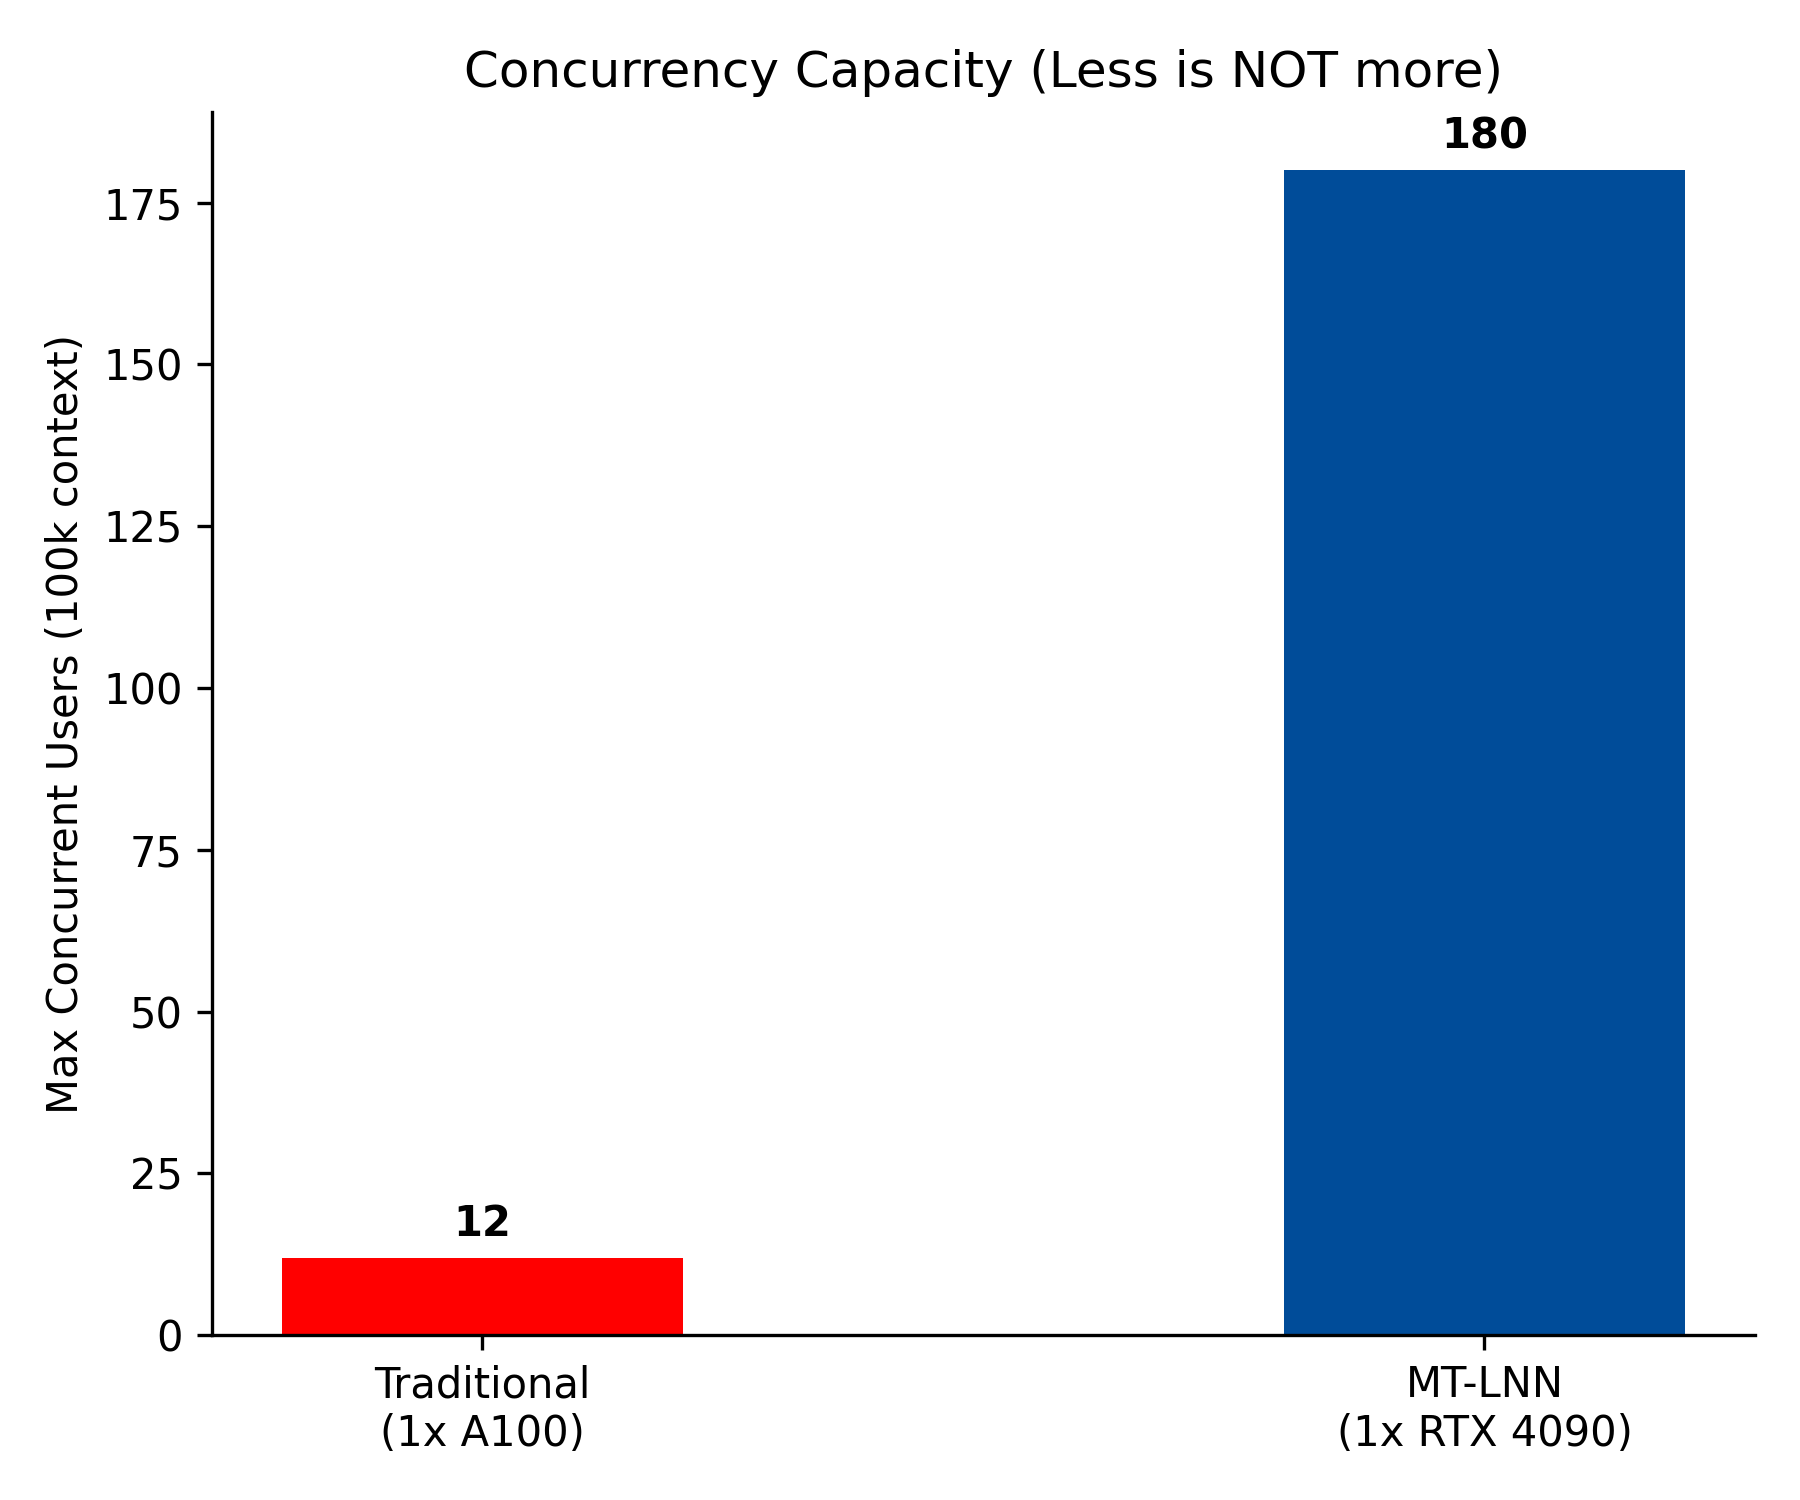
\includegraphics[width=\textwidth]{concurrency.png}
\end{column}
\begin{column}{0.5\textwidth}
\centering
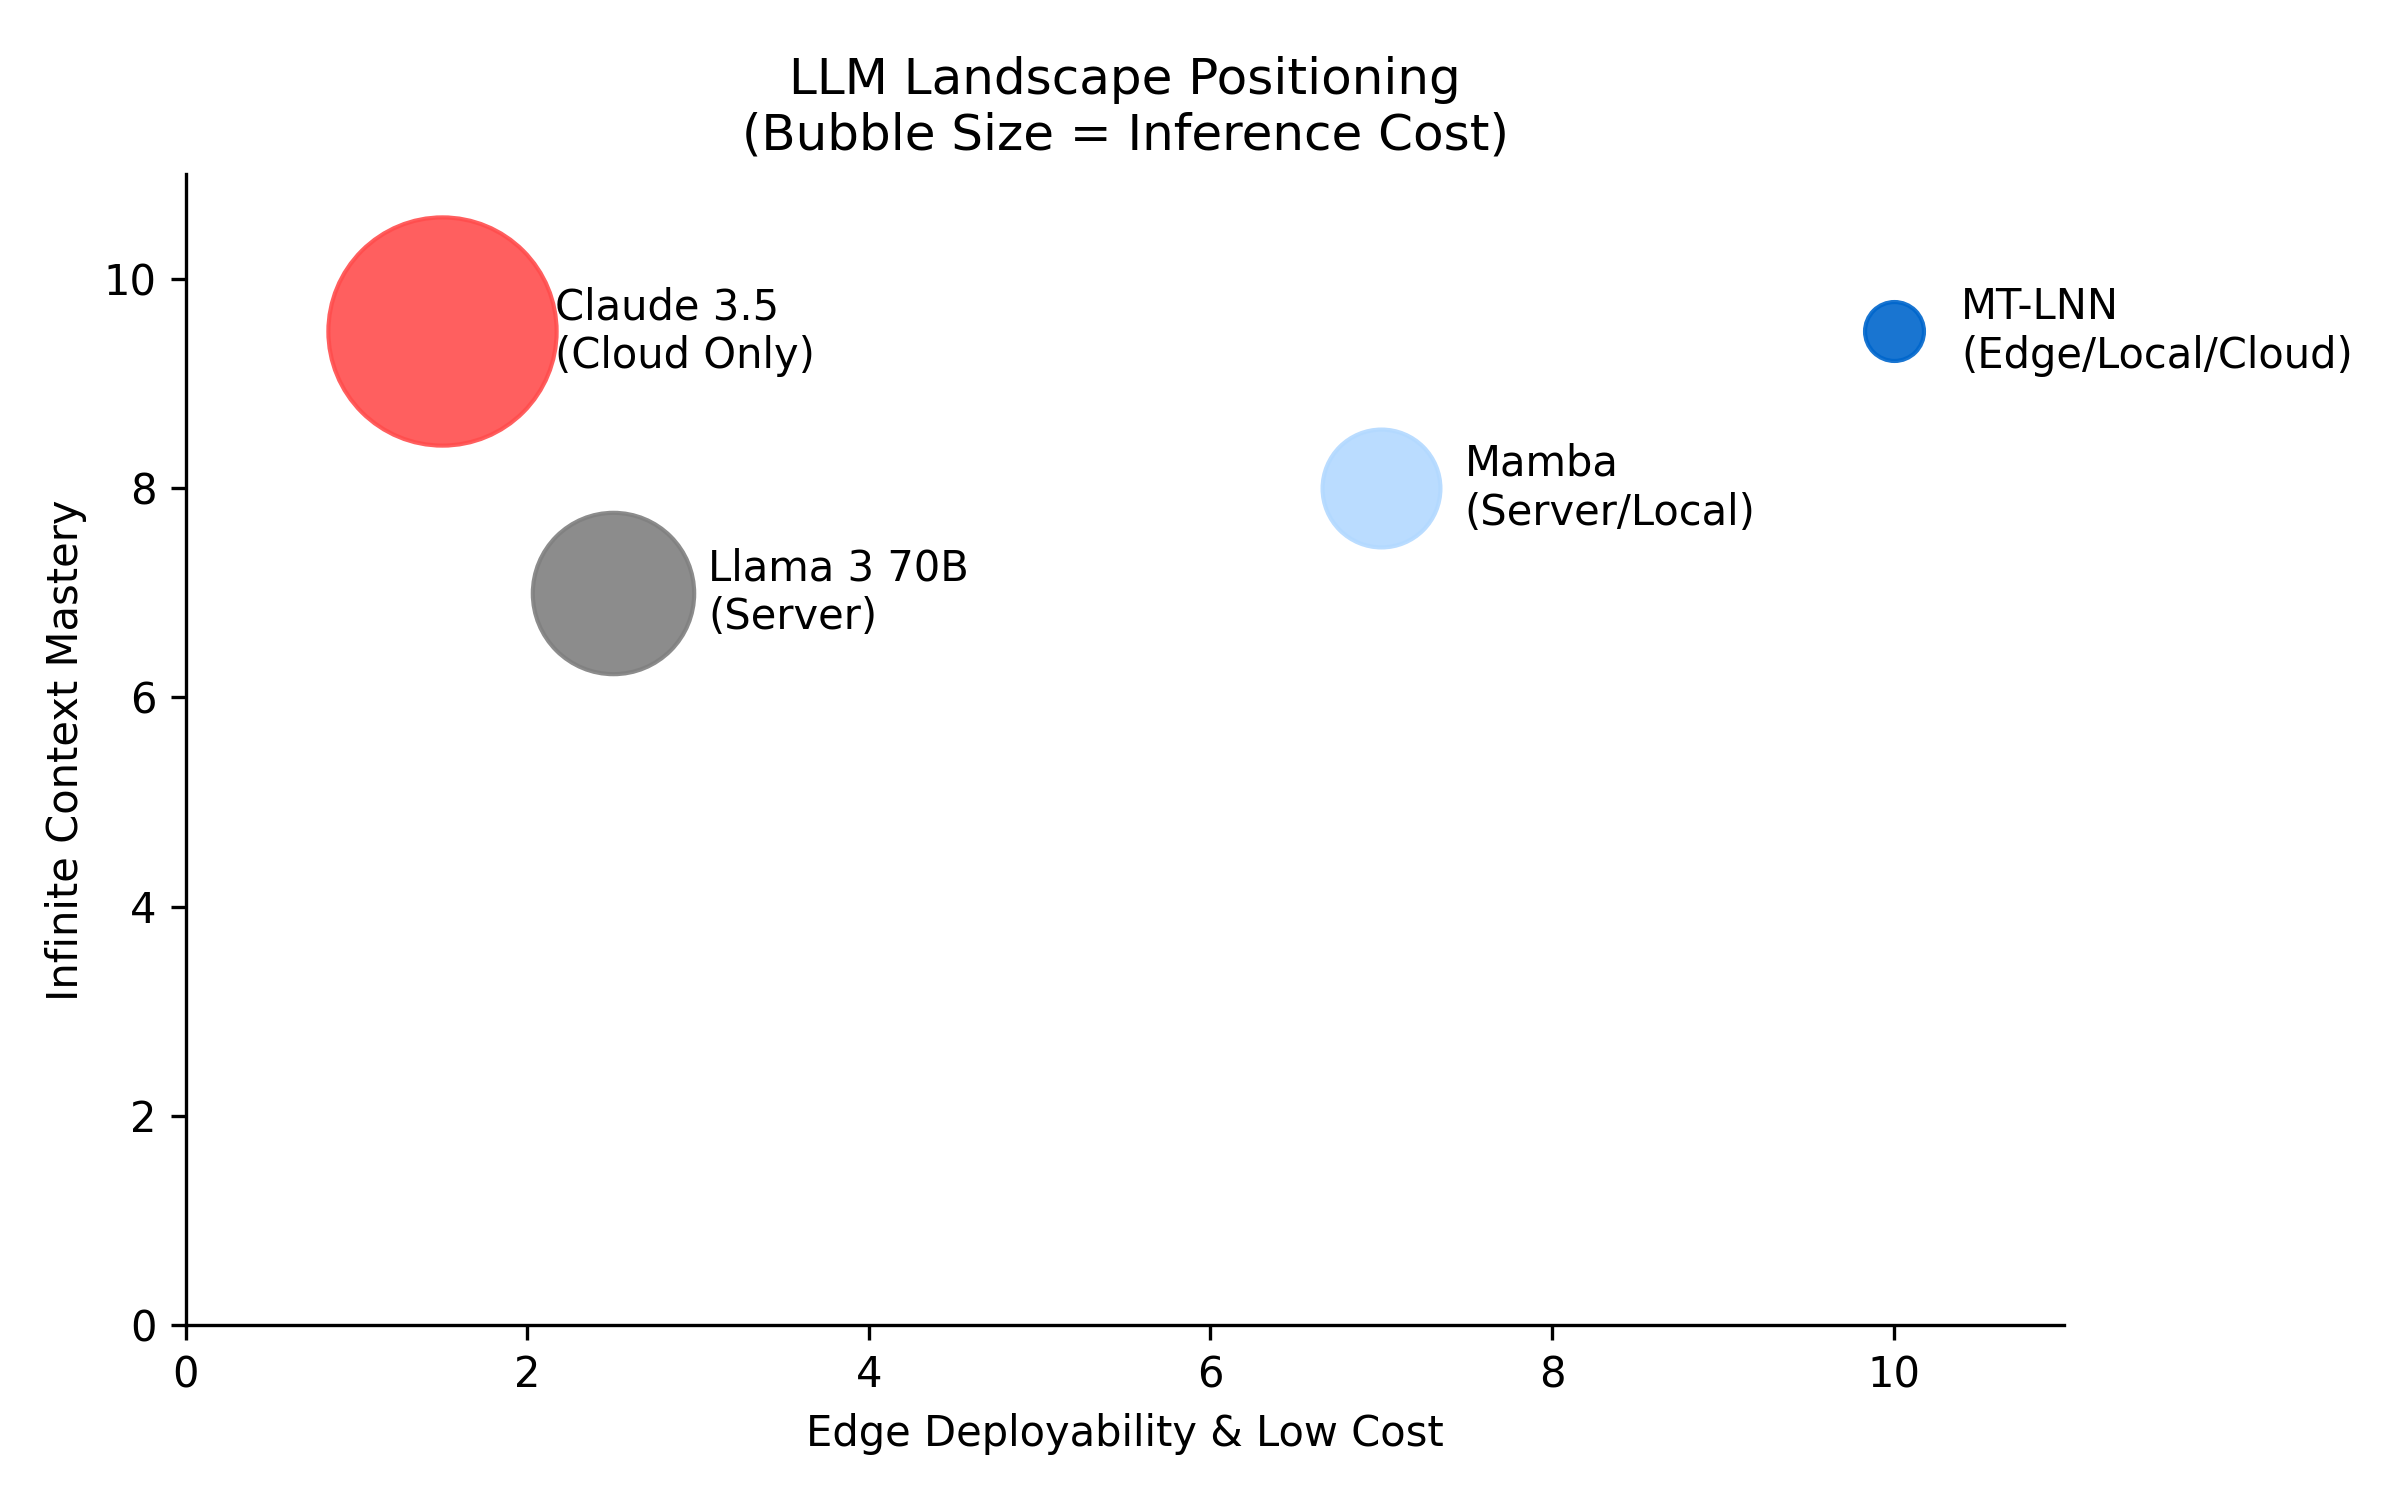
\includegraphics[width=\textwidth]{landscape.png}
\end{column}
\end{columns}
\end{frame}

\begin{frame}{高并发与 TCO (整体拥有成本) 优势}
\begin{itemize}
    \item \textbf{规模性降低推理成本：} 由于摒弃了呈二次方膨胀的 KV 缓存矩阵，千字大段输入与短语指令在 MT-LNN 中的运行内存消耗基本一致。预计云端模型的大规模服务算力成本可降低至现有方案的 1/10。
    \item \textbf{处理极端并发场景表现卓越：} 
        若同时应对 100 用户各 10 万字级别的极限请求推送：普通 A100 模型集群极可能因显存激增而导致 OOM（宕机崩溃）；而我们可仅用单台消费级加速显卡从容稳定排队并行反馈。
\end{itemize}
\end{frame}

\begin{frame}{蓝海下沉市场 1：IoT 与边缘嵌入设备}
\begin{itemize}
    \item \textbf{解决物理芯片发热与功耗瓶颈：} 模型不仅体积小，而且对内存读写的极速优化使得我们能将其无缝嵌入到功耗受限的可穿戴 AR 交互外设和车载中枢内。
    \item \textbf{全天候陪伴式流信息处理：} 现存主流 AI 无法承载几十小时全时段开启音视频输入捕捉，而 MT-LNN 随时间递进的连续动态吸收机制天然适用这类连绵不断的外界数据流场景。
\end{itemize}
\end{frame}

\begin{frame}{商业落脚点 2：B 端垂直机构与研发刚需}
\begin{itemize}
    \item \textbf{B 端目标客户痛点吻合：} 
        顶尖律所面临海量千页卷宗的溯源；风投/审计财团对无尽财报报表的数据对齐；或大型科技厂商进行的底层百万行老旧祖传代码库盘查检越。
    \item \textbf{三要素完美匹配：} MT-LNN 精准满足这部分客户迫切需求的三个必要条件：1. 超长篇幅大批量吞吐能力。2. 绝对的私有合规和不联网隔离。3. 基于极低硬件投入的一次性低成本本地部署。
\end{itemize}
\end{frame}

\begin{frame}{当前进展：成熟的长文本 RAG Demo 演示}
\begin{itemize}
    \item \textbf{工程化验证进度稳健：} 目前技术不仅具备深厚的理论与论文基础验证，且已实现完整的模型级封装工程化。我们结合了最新组件搭建了流畅运作的大规模文档推理前端平台。
    \item \textbf{优秀的交付适应性：} Demo已完成标准化装箱打包测试。能即刻满足本地脱网部署演示要求，或快速封装成微服务流交付并入传统企业的已有网络中，打通产品化最后一公里。
\end{itemize}
\end{frame}

\begin{frame}{核心技术路线与 18 个月展望}
\begin{enumerate}
    \item \textbf{一阶段验证期 (当前)：} 在极小参数级模型（如挂载架构至 1.5B 参数量级规模）下，初步获得行业内长文本测评榜单领先与学术验证，并吸引第一梯队种子与社区开发者讨论。
    \vspace{0.5em}
    \item \textbf{二阶段架构规模化 (随后的 6-12 个月内)：} 着手引入充足起步的高算力集群资源，开发训练并推出完全原生结构的大规格 7B (70亿) 级底层大模型组件架构。与初期 B 端合作伙伴深度联合开发落地闭环体系与行业最佳实践案例。
    \vspace{0.5em}
    \item \textbf{三阶段迈向下一代泛化多模态基座 (未来 18 个月以上)：} 跨越多模态，使用超千亿宏大数据集参与大规模通用联合训练。并用该极致常数时间效能最终推动更高度的泛化 AGI 理解引擎构建计划底座。
\end{enumerate}
\end{frame}

\begin{frame}{融资方案与阶段目标 (The Ask)}
\begin{columns}
\begin{column}{0.5\textwidth}
\textbf{本轮诉求：Seed / A 轮 - \$3.5M}
\vspace{0.5em}
\begin{itemize}
    \item 启动 7B 级原生大模型基座训练环境。
    \item 组建成熟的 GTM 和企业级销售团队。
    \item \textbf{12个月里程碑（非营收承诺）：}
    \begin{itemize}\footnotesize
        \item 与 $\geq$ 10 家高德企业/机构签约 着合作备忘录 / PoC。
        \item 其中 3--5 家转为付费 design partner，建立可验证的付费需求信号。
        \item 发布第一个生产环境可用 7B 检查点 + 公开 benchmark 报告。
    \end{itemize}
\end{itemize}
\end{column}
\begin{column}{0.5\textwidth}
\textbf{资金使用占比：}
\begin{itemize}
    \item \textbf{50\% 算力与预训练：} 租赁 H100 / A100 集群跑 7B 基座联合预训练。
    \item \textbf{30\% LNN 核心研究：} 拓充连续时间动力学 (LTC ODE)、Orch-OR 启发选择机制、工作记忆 GWTB 方向的研究人员，差异化的技术周边护城河在这里。
    \item \textbf{20\% GTM 与市场：} B 端客户销售 + 社区 / 论文 / 品牌。
\end{itemize}
\end{column}
\end{columns}
\end{frame}

\begin{frame}{核心团队：Awareness}
\begin{itemize}
    \item \textbf{Everest An -- 创始人} (前沿计算系统与神经网络架构师)
    \vspace{0.5em}
    \item \textbf{去中心化基建经验：} 前 \textbf{IPFS Athna} 核心成员，曾主导并全面负责中国地区企业级分布式数据库的底层架构建设。
    \item \textbf{头部资本与生态视角：} 曾任出海顶级基金 \textbf{Outliers Fund} 投资管理经理。重点参与投资顶尖公链体系 (\textbf{Dfinity}、\textbf{Harmony})、前沿基础设施 (\textbf{Analog})，及区块链核心代码安全审计机构 (\textbf{Quantstamp})。
    \item \textbf{顶级开发者底色：} 具备全球顶尖的工程技术实力，在竞争最激烈的全球以太坊 (\textbf{Ethereum}) 黑客马拉松大赛中多次斩获冠军。
\end{itemize}
\end{frame}

\begin{frame}{我们真正的技术护城河}
\small
\begin{itemize}\itemsep=0.5em
    \item \textbf{架构原创性（最深的一层）：} MT-LNN 本身——连续时间 LTC ODE + Orch-OR 启发的选择机制 + GWTB 工作记忆三件套——是我们的原创架构，论文在投稿中。架构本身是不可被快速复现的原创资产。
    \item \textbf{可复现的训练 recipe 与跨基座经验：} 从 Qwen-0.5B 到 Qwen-3B、Llama 多个基座上的 adapter 训练数据、超参与消融报告均已沉淀在仓库。后来者即使拿到架构，也需数月 reproduce 这一套经验。
    \item \textbf{Benchmark 与评测体系：} 大海捞针 / 选择性拷贝 / O(1) 内存压力测试 / 稀疏共振消融，全部自研、公开、可复现。
    \item \textbf{开源社区 + 早期 design partner 飞轮：} 代码、权重、反馈闭环先发。Mamba / RWKV 都是靠这一招拉开差距。
\end{itemize}
\end{frame}

\begin{frame}{结语}
\begin{itemize}
    \item \textbf{传统算力困境遭遇瓶颈：} 模型发展正处于极度内卷的瓶颈期，单纯的堆砌算力带来的边际收益已大幅降低。仅靠扩大集群无法从根本上跨越内存功耗痛点墙。
    \item \textbf{底层流机制的范式转移：} 转向更具生物启发性质与动态内状态循环记忆能力的架构才是彻底解构目前“高成本困境长城”的根本有效破局路径。
    \item \textbf{绝佳的时间节点：} 项目当前不仅仅具备完善的跨时代理论架构支撑，同时辅以充分完备的大批量基础对比论证代码及可跑的测试验证案例。现在正是投资这一新型赛道的黄金入局契机。
    \vspace{0.5em}
    \item \textit{Invest in Awareness. Invest in the Liquid Computing Paradigm Shift.}
\end{itemize}
\end{frame}

\begin{frame}{联系方式与相关主页}
\begin{center}
    \LARGE \textbf{Awareness} \\
    \vspace{0.5em}
    \large Everest An -- 创始人 / 核心架构师 \\
    \vspace{1.5em}
    \normalsize
    \textbf{Email:} everest9812@gmail.com \\
    \textbf{WeChat / Telegram:} EverestAn \\
    \vspace{1.5em}
    \small
    \textbf{论文 (Paper):} \url{https://huggingface.co/EverestAn/MT-LNN} \\
    \textbf{代码 (GitHub):} \url{https://github.com/everest-an/M1} \\
    \textbf{在线演示 (Demo):} \url{https://huggingface.co/spaces/EverestAn/AwarenessO1} \\
    \vspace{1.5em}
    \textit{欢迎交流，共同探索下一代液态算力革命。}
\end{center}
\end{frame}

\end{document}



